\documentclass[11pt]{article}
\usepackage[letterpaper,margin=.83in]{geometry}
\usepackage[T1]{fontenc}
\usepackage{lmodern,microtype,graphicx,booktabs,amsmath,amssymb,array,hyperref,fancyhdr,caption}
\hypersetup{hidelinks,pdftitle={An outside statistician's reading of the HPS significance studies}}
\pagestyle{fancy}\fancyhf{}\setlength{\headheight}{14pt}
\fancyhead[L]{\small HPS-GPR: a fresh statistical reading}\fancyhead[R]{\small 21 September 2026}\fancyfoot[C]{\thepage}
\setlength{\emergencystretch}{2em}\captionsetup{font=small}
\begin{document}
\begin{center}{\LARGE\bfseries What looks interesting, and what\\more 2021 data could settle}\par\vspace{7pt}
{\large An outside statistician's reading of v5.0.5 and the v5.8 series}
\end{center}
\noindent\textit{Perspective: I approach these records as a statistician concerned with background modeling at high event counts. I take the supplied detector response and event selections as assumptions to be checked, not as established facts of my own. This is a review of saved results; no new fits are performed.}

\section*{My judgement}
Yes, I find enough structure here to justify a carefully designed replication. I do not yet find the combined result persuasive evidence for a new particle. I would prioritize 90--93 MeV and 65--67 MeV, for different reasons. The former is the most interesting question about consistency across datasets; the latter is the cleaner candidate under the analysis's actual common-coupling hypothesis. Neither currently has strong, background-independent global evidence.

My main reservation is that the combined feature becomes stronger when the physical relationship between the dataset amplitudes is relaxed. A common location and a common physical signal rate are different claims. The value of more 2021 data is that it can test that distinction.

\begin{table}[h]\centering\small
\begin{tabular}{p{.17\linewidth}p{.75\linewidth}}\toprule
Region & My assessment\\\midrule
90--93 MeV & First priority for replication and rate consistency. Free nonnegative amplitudes give conditional local/global $Z=3.583/2.060$ at 92 MeV; the direct global check has 7/256 exceedances. Fisher and Stouffer also prefer 92 MeV, but reuse the same events.\\[4pt]
65--67 MeV & The common-coupling fit's preferred region. At 66 MeV all three raw fitted roots are positive. The v5.8.4 reference-local $Z=2.829$ becomes only $0.812$ globally. A sensible target, with weak current evidence.\\[4pt]
51 MeV & Primarily a 2015 residual to understand. Its raw root is 3.139, versus $-0.367$ in 2016 and 0.234 in 2021 at that mass; the shared root is 1.221. Cross-campaign support is limited.\\[4pt]
76--80 MeV & Track the ordinary 2021 peak near 78 MeV, but treat the spectacular 76 MeV stress-centered score as a model diagnostic. At 76 MeV the 2016 raw root is $-2.46$ and the combined root is only 0.166.\\\bottomrule
\end{tabular}
\caption{Priorities for follow-up, not a new ranking by calibrated discovery probability. The quoted v5.8 combined results use the full declared search and $\pm2.25\sigma_m$ masks. Different rows are not independent tests.}
\end{table}

\section*{What I mean by ``interesting''}
The 92 MeV feature survives modest width variations and several ways of combining the datasets. That earns attention, but not independent confirmations: these are repeated views of the same spectra. The earlier coherence test gives a lower-tail probability about 0.763, so the observed clustering is not unusually tight under that conditional null. I would regard this as a useful, falsifiable candidate rather than an emerging discovery.

\clearpage
\section*{Does the fixed-background combination look interesting?}
The answer depends on what is fixed. The v5.8 studies freeze a \emph{generating spectrum} for the toys, while retraining the masked GP and profiling its background uncertainty in each extraction. This is an informative conditional calculation. It is the combination I would retain as a starting point for follow-up, with its source assumptions stated.

A likelihood that instead treats the estimated background as perfectly known sets its nuisance covariance to zero. I would not give a stronger-looking curve extra evidential weight merely because it does that. In the note's 41-mass common-range calibration, the median fixed/profiled observed-limit ratio changes from 0.595 before calibration to 1.346 afterward. Those are \emph{limit ratios}, not significance ratios, but they show why an apparent advantage from omitting uncertainty is not automatically real. I did not recover a verified fixed-covariance combined discovery scan, so I do not assign it a peak significance here.

\begin{figure}[h]\centering
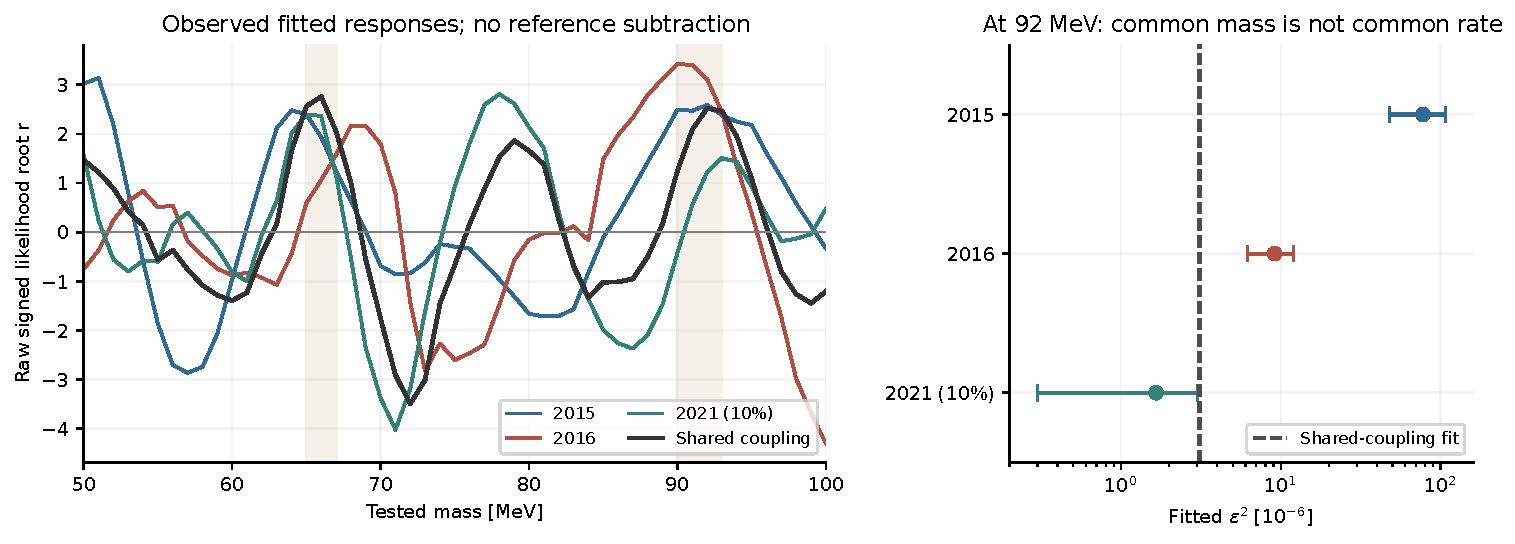
\includegraphics[width=\linewidth]{../figures/observed_evidence.pdf}
\caption{Saved v5.8.4 baseline fits, with GP background uncertainty profiled. Left: raw signed roots, without reference centering. Shading marks the two principal follow-up regions. Right: individual coupling-squared estimates at 92 MeV, using the inherited conversion; bars are conditional local fit standard errors. The dashed line is the shared-coupling estimate. The horizontal scale is logarithmic. These bars do not include all detector or normalization uncertainties and are not a calibrated compatibility test.}
\end{figure}

At 92 MeV the individual fitted $\epsilon^2$, in units of $10^{-6}$, are
\[
77.48\pm29.96\quad(2015),\qquad
9.13\pm2.93\quad(2016),\qquad
1.65\pm1.35\quad(2021).
\]
The positive excursions therefore do not automatically describe one common rate. The shared-coupling raw root is 2.520 there, whereas allowing three nonnegative amplitudes produces the more prominent combined feature. The rate conversions themselves need qualification before this difference becomes a physical inconsistency claim.

The present 2021 sample supplies about 82\% of the local null information in the shared fit at 92 MeV, but its raw root is only 1.222. This explains why the common-coupling result is more modest: it is strongly constrained by the most precise dataset. At 66 MeV the corresponding 2021 information share is about 55\%, and the raw roots are 1.934, 1.061 and 2.366. I would keep both hypotheses; I would not select a combination method because it makes one of them look strongest.

\clearpage
\section*{What additional 2021 events could clarify}
\textbf{First, test replication in genuinely new events.} If a later total includes the currently examined 10\%, analyze its additional events separately before showing the pooled result. Freeze the mass hypotheses, background policy, resolution model, signal statistic and $\pm2.25\sigma_m$ mask beforehand. A search within each nominated interval still has a trials correction, as does choosing among the nominated candidates. The earlier events are useful for defining those predictions; they are not an independent confirmation of them.

\textbf{At 90--93 MeV, test the amplitude as well as the mass.} The most discriminating question is whether new 2021 events support a resolution-shaped excess at the rate predicted by a qualified common-coupling model. Better precision could strengthen that model, or show that the older residuals cannot share its rate. A reproducible but discrepant rate could instead point to a normalization, acceptance or background-model issue. The current weak 2021 response makes this comparison particularly useful.

\textbf{At 65--67 MeV, test the actual combined preference.} This is the region the physically restricted combination selects. A matching fractional excess in new 2021 data would justify a combined assessment with the fixed analysis. Its disappearance would be informative too. Around 76--80 MeV I would also examine the neighboring residual pattern: the moving background fit can turn a peak in one window into an apparent deficit in another. Such neighbors must not be counted as independent corroboration.

\textbf{More counts do not by themselves settle background adequacy.} If a background error has a fixed fractional shape, its residual scales with exposure just as a real signal fraction does. In a simple counting approximation,
\[
 Z_{\rm mismatch}(k)\simeq
 \frac{k\,\delta b}{\sqrt{k\,b}}
 =\sqrt{k}\,\frac{\delta b}{\sqrt b}.
\]
A growing nominal significance can therefore diagnose an increasingly visible modeling error. I would compare fractional residuals, the expected peak width, sideband behavior and justified control selections. Source uncertainty and signal absorption during source building must be included in that assessment. The additional sample can reject a chance fluctuation; distinguishing persistent background structure from a particle requires these further checks.

\textbf{The existing full-exposure projections are scenarios, not predictions.} The v5.0.5 projection chapter assumes persistence of selected partial-sample excesses; its 78 MeV target of 8.88 follows that assumption, and the matched-injection construction is adjusted to reproduce the chosen scaling. I would not quote that number as the expected significance of unseen data. A selected upward fluctuation has an upward-biased amplitude estimate, and a learned background need not follow the known-background $\sqrt{k}$ rule.

\section*{What would change my mind}
I would be substantially more interested after a predeclared new-data test found the predicted mass, width and rate, with acceptable background residuals and demonstrated calibration of the complete source-building procedure. An increase in a fixed-background score alone would not be enough. My present conclusion is positive about doing the replication and cautious about the current particle interpretation.

\vfill
\noindent{\footnotesize\textbf{Evidence and scope.} Sources: v5.0.5 Sections 4.20/6.11, its calibration appendix and full-2021 projection chapter; v5.8.2 raw/reference scans; v5.8.4 baseline combination and amplitude ledgers; v5.8.5 free-amplitude and coherence results. Reference-local and global scores remain conditional on frozen, observed-data-derived source spectra. The full source list, hashes, numerical rows and two specialist reviews accompany this report. No new fit, significance calibration or exposure forecast was produced.}
\end{document}
